\documentclass{standalone}

\usepackage{tikz}
    \usetikzlibrary{arrows.meta}
    \usetikzlibrary{calc}
    \usetikzlibrary{decorations.pathmorphing}

\tikzset{
    greensq/.style={
        black!90,
        fill=green!40, 
        line width=0.4mm,},
    redsq/.style={
        black!90,
        fill=red!40, 
        line width=0.4mm,},
    }
    
\begin{document}
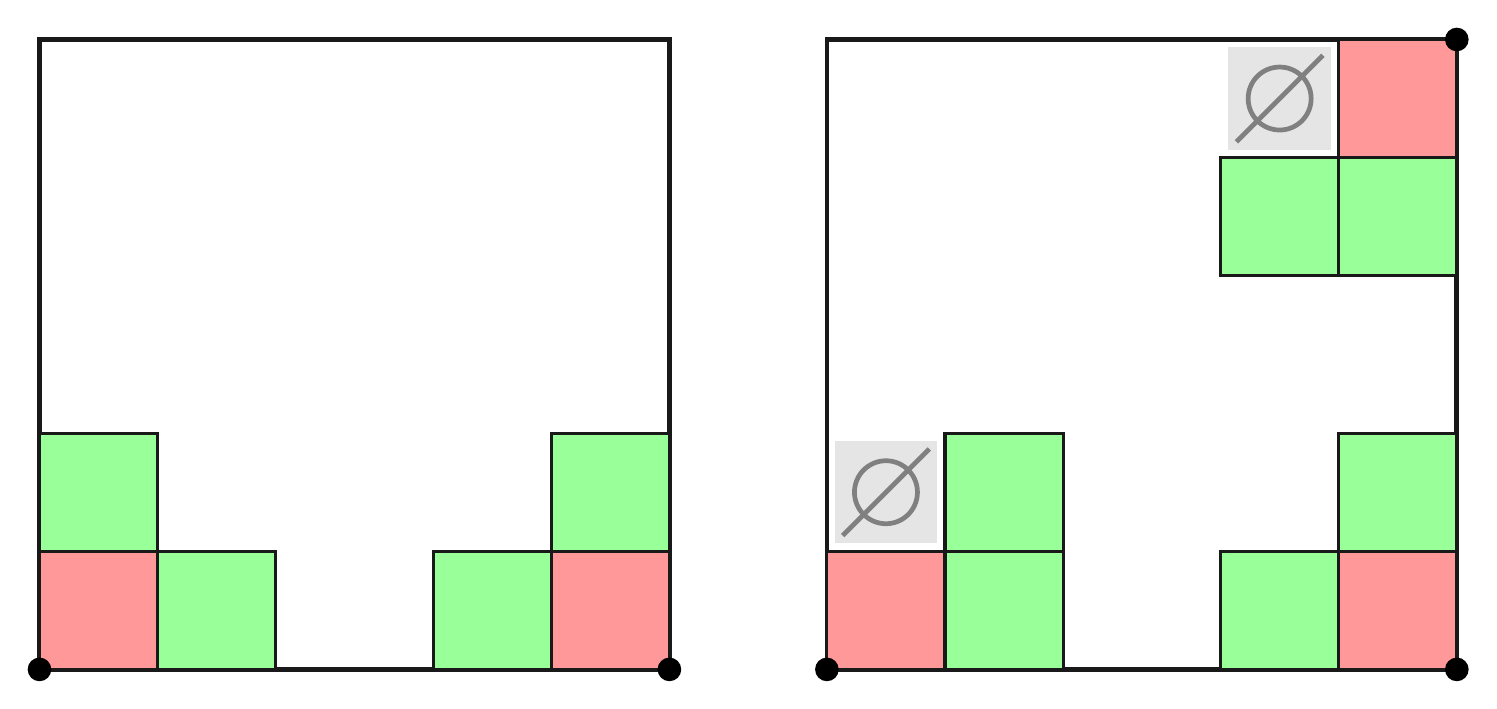
\begin{tikzpicture}
    % \draw[help lines] (0,0) grid (15,3);
    \foreach \x in
        {(0,0),(10,0)} 
        {\draw[black!90, line width=0.6mm] \x rectangle+(8,8);}
    \foreach \x in
        {(0,0), (6.5,0), (10,0), (16.5,0), (16.5,6.5)} 
        {\draw[redsq] \x rectangle+(1.5,1.5);}
    \foreach \x in
        {(0,1.5), (1.5,0), (5,0), (6.5,1.5), 
         (11.5,1.5), (11.5,0), (15,0), (16.5,1.5), (15,5), (16.5,5)} 
        {\draw[greensq] \x rectangle+(1.5,1.5);}
    \foreach \x in
        {(10,1.5), (15,6.5)} 
        {\fill[black!10] \x++(0.1,0.1) rectangle+(1.3,1.3);
         \draw[black!50, line width=0.6mm,] 
            \x++(0.2,0.2) -- +(1.1,1.1)
            \x++(0.75,0.75)circle(0.4);}
    \foreach \x in
        {(0,0), (8,0), (10,0), (18,0), (18,8)}
        {\fill[black] (\x circle (1.5mm);}
\end{tikzpicture}
\end{document}